\section{Block Codes and Hamming Distance}\label{section_1.1}

\begin{definition}
  We define an \textbf{alphabet} to be an arbitrary finite set $Q$ of size $q$,
  whose elements we call \textbf{symbols}. Given some $n \in \Z^+$, we call
  elements of $Q^n=\underbrace{Q \times \dots \times Q}_{n\text{-times}}$
  \textbf{words} or \textbf{strings} in the alphabet.
\end{definition}

\begin{example}\label{example_1.1}
  \begin{enumerate}
    \item[(1)] The standard English alphabet
      \begin{align*}
        A B C D E F G H I J K L M N O P Q R S T U V W X Y Z \\
      \end{align*}
      is an alphabet of size $26$. A word in this alphabet can be the words
      ``DOG'' and ``COOKED'' as well as the word ``AFDAFDKAJFDAJFA''.

    \item[(2)] The \textbf{binary field} $\F_2=\{0,1\}$  (i.e. the finite field
      on two elements) is an alphabet of size $2$. Likewise, the
      \textbf{ternary field} $\F_3=\{0,1,2\}$ where $2 \equiv -1 \mod{3}$ is an
      alphabet of size $3$. We define the  \textbf{$q$-ary field} to be the
      finite field $\F_q$ on $q=p^r$ elements, where  $p,r \in \Z^+$ and $p$ is
      prime.

    \item[(3)] The fields $\R$ and $\C$ are not alphabets, since they are not
      finite sets; they are not even countable sets. The sets $\Q$ and $\Z$ and
      $\N$ are also not alphabets, they are countable, but not finite.
  \end{enumerate}
\end{example}

\begin{definition}
  Let $Q$ be an alphabet of size $q$. We define a \textbf{code} $C$ to be any
  collection of words in $Q$, and we call the elements of $C$
  \textbf{codewords}. If $C \subseteq Q^n$, then we call $C$ a  \textbf{block
  code} of \textbf{length} $n$.
\end{definition}

\begin{example}\label{example_1.2}
  \begin{enumerate}
    \item[(1)] The collection $\{\text{``DOG''}, \text{``CAT''},
      \text{``GOOSE''}\}$ is a code in the english alphabet, but it is not a
      block code. The code $\{\text{``DOG''}, \text{``CAT''},
      \text{``HAT''}\}$ is a block code of length $3$ in the english alphabet.

      \item[(2)] In $\F_2$, the codewords  $11001111$ and  $101011$ form a code
        in  $\F_2$ but not a block code. The codewords $11111$, $00000$,
        $11001$, and  $10101$ form a block code of length  $5$ in  $\F_2^5$.

      \item[(3)] We define the \textbf{$q$-ary repitition code} to be the image
        of the following map $\F_q \xrightarrow{} \F_q^n$ taking $i
        \xrightarrow{} (i, \dots, i)=i \dots i$. That is we take any symbol in
        $\F_q$ and repeat it $n$ times. This code is a block code of length $n$
        in $\F_q^n$.
  \end{enumerate}
\end{example}

\begin{definition}
  Let $Q$ be an alphabet. We define the  \textbf{Hamming distance} of two words
  $x,y \in Q^n$ to be the number of coordinates in which they differ; i.e. if
  $x=(x_1, \dots, x_n)$, and $y=(y_1, \dots, y_n)$, then:
  \begin{equation}\label{equation_1.1}
    d(x,y)=|\{i : x_i \neq y_i\}|
  \end{equation}
  We define the \textbf{Hamming weight} of a word $x \in Q^n$ to be the number
  of nonzero positions in $x$:
  \begin{equation}\label{equation_1.3}
    w(x)=d(x,0)
  \end{equation}
  Where $0 \in Q^n$ is the word consisting of all $0$.
\end{definition}

\begin{lemma}\label{lemma_1.1.1}
  The Hamming distance defines a metric on any alphabet.
\end{lemma}
\begin{proof}
  Let $Q$ be any alphabet, and  $x,y,z \in Q^n$ be words. Observe by equation
  \ref{equation_1.1} that we have a map $d:Q^n \times Q^n \xrightarrow{} \N$, so
  that $d(x,y) \geq 0$. Now, we also have that $d(x,y)=0$ if, and only if
  $x_i=y_i$ for all  $1 \leq i \leq n$, if and only if $x=y$. Moreover, we also
  notices that  $d(x,y)=d(y,x)$, since the difference in position does not
  depend in the order in which we compare.

  Now, suppose that $d(x,y)=l$ and $d(y,z)=k$, then $x$ and  $y$ differ in  $l$
  positions, and  $y$ and $z$ differ in $k$ positions. Therefore, $x$ and $z$
  must differ in at most  $l+k$ positions so that  $d(x,z) \leq
  l+k=d(x,y)+d(y,z)$.
\end{proof}

\begin{definition}
  We define the \textbf{minimum Hamming distance} of a code $C$ to be
  \begin{equation}\label{equation_1.3}
    d=\min_{x,y \in C}{\{d(x,y) : x \neq y\}}
  \end{equation}
  We define the \textbf{minimum Hamming weight} of $C$ to be:
  \begin{equation}\label{equation_1.4}
    w=\min_{x,y \in C}{\{w(x) : x \neq 0\}}
  \end{equation}
\end{definition}

\begin{definition}
  Let $Q$ be an alphabet and  $C \subseteq Q^n$ a block code of length $n$. We
  define the  \textbf{covering radius} of $C$ to be the smallest postive integer
   $\r$ for which the balls $B_\r(c)$ cover $Q$, for all $c \in Q$. We define
   the \textbf{sphere packing radius} of $C$ to be the largest positive integer
    $\e$ for which the balls $B_\e(c)$ are disjoint for every $c \in C$.
\end{definition}

\begin{lemma}\label{lemma_1.1.2}
  Let $C$ be a block code with sphere packing radius $\e$ and covering radius
  $\r$. Then the minimum distance of  $C$ is either  $2\e+1$ or  $2\e+2$, and
  \begin{equation}\label{equation_1.5}
    \r=\max{\{\min{\{d(x,c) : c \in C\}} : x \in Q^n\}}
  \end{equation}
\end{lemma}
\begin{proof}
  We have that for any $c, c' \in C$, that $2\e<d(c,c')$. Indeed, suppose not,
  that $d(c,c') \leq 2\e$. Choose an $x \in B_\e(c)$, then $d(x,c) \leq \e$ so
  taht we get by the triangle inequality $2\e-d(x,c') \leq \e$, so that $d(x,c')
  \leq \e$ which puts $x \in B_\e(c')$. But that contradicts the definition if
  $\e$ as the sphere packing radius.

  Now, we have that since $2\e<d(c,c')$ for all $c,c' \in C$, letting $d$ be the
  minimum distance of  $C$,  $2\e<d$. This makes $2\e+1 \leq d$. Now, suppose
  that $x,y \in C$ for  which $2\e+1 \leq d \leq d(x,y)$. Then $x$ and $y$ must
  differ in at least $2\e+2$ places, for if they differ in  $2\e+1$ places, we
  contradict that  $d$ is the minimum distance. therefore we get that  $2\e+1
  \leq d \leq 2\e+2$.

  Now, let $x \in Q^n$, and let $c \in C$ for which $x \in B_{\r_{\a_1}}(c)$,
  choose another $c' \in C$ for which $x \in B_{\r_{\a_2}}(c')$. Then we observe
  that $d(x,c) \leq \r_{\a_1}$ and $d(x,c') \leq \r_{\a_2}$. Now, let
  \begin{equation*}
    S_x=\{\r_{\a_i} : d(x,c) \leq \r_{\a_i} \text{ for all } c \in C\}
  \end{equation*}
  and take $\r_\a(x)=\sup{S_x}$. Such a $\r_\a(x)$ exists since each $r_{\a_i}$
  is a positive integer. Then observe that $\r=\inf_{x \in Q^n}{\{\r_\a(x)\}}$.
  This gives us equation \ref{equation_1.5}.
\end{proof}

\begin{figure}[h]
  \centering
  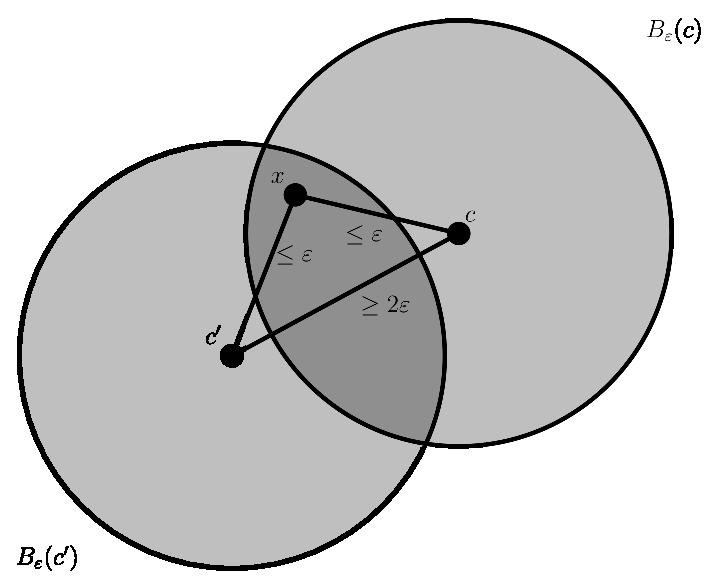
\includegraphics[scale=0.5]{Figures/Chapter1/sphere_packing.eps}
  \caption{The Sphere packing radius of the code $C$}
  \label{figure_1.1}
\end{figure}

\begin{figure}[h]
  \centering
  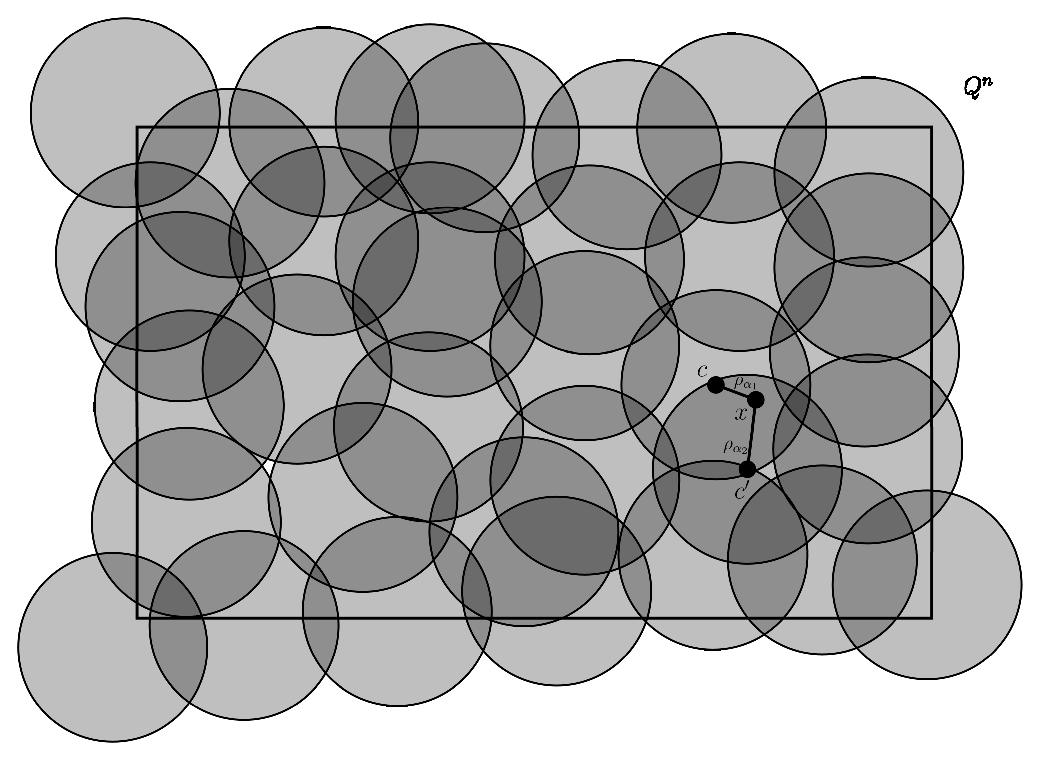
\includegraphics[scale=0.5]{Figures/Chapter1/covering_radius.eps}
  \caption{The Covering radius of the code $C$}
  \label{figure_1.1}
\end{figure}

\begin{definition}
  Let $C$ be a block code with sphere packing radius  $\e$ and covering radius
  $\r$. We call  $C$ a  \textbf{perfect code} if $\e=\r$.
\end{definition}

\begin{example}\label{example_1.3}
  Let $Q$ be any alphabet, and $C$ a block code of length $n$ in $Q$. If
  $|C|=1$, then we call  $C$ the  \textbf{trivial block code}, or the
  \textbf{trivial code}. Observe that since the trivial code consists only of
  one code word, then the sphere packing radius and the covering radius
  coincide. That is trivial codes are perfect, however, there is no notion of
  minimum distance in a trivial code since there is only one codeword.
\end{example}

\begin{definition}
  We call a block code $t$-\textbf{error correcting} if for any nonzero
  codewords $c$ and $c'$, and for any codewords $x,y$ of Hamming weight  $w(x)
  \leq t$ and $w(y) \leq t$ we have
  \begin{equation*}
    c+x \neq c'+y
  \end{equation*}
\end{definition}

\begin{theorem}\label{theorem_1.1.3}
  A block code $C$ with minimum distance $d$ is $t$-error correcting if, and
  only if  $d \geq 2t+1$.
\end{theorem}
\begin{proof}
  Suppose that $d \geq 2t+1$; i.e. $d>2t$. Let $c,c' \in C$ be nonzero
  codewords, and choose $x,y \in C$ with $w(x) \leq t$ and $w(y) \leq t$ for
  which $c+x=c'+y$. Then $x-y=c-c'$, and we get $w(x-y)=w(c-c')=d(c,c') \leq
  2t<d$ which contradicts that $d$ is the minimum distance.

  Now, suppose that  $d<2t+1$, so that $d \leq 2t$, and let $c \in C$ a codeword
  of weight $w(c)=d$. Now, define the codeword $c' \in C$, obtained from $c$ by
  setting $\lceil \frac{d}{2} \rceil$ non-zero positions to $0$. Then we observe
  that  $w(c') \leq d-\lceil \frac{d}{2} \rceil<=t$, and $w(c-c')=d(c,c')=
  \lceil \frac{d}{2} \rceil \leq t$, but that $c'+0=c+(c-c')$, so that $C$
  cannot be  $t$-error correcting.
\end{proof}
